\documentclass{beamer} 
\usepackage[utf8]{inputenc}
\usepackage[T1]{fontenc}
\title{Powierzchnia Seiferta, genus i suma spójna węzłów}
\date{03.04.2024}
\author{Weronika Jakimowicz}

\usetheme{texsx}

\uselanguage{polish}
\languagepath{polish}
\deftranslation[to=polish]{Definition}{Definicja}
\deftranslation[to=polish]{Theorem}{Twierdzenie}

\usepackage{tikz}
\usetikzlibrary{calc, intersections, knots}

\usepackage{pgfplots}

\AtBeginSection[]{
  \begin{frame}
  \vfill
  \centering
  \begin{beamercolorbox}[sep=8pt,center,shadow=true,rounded=true]{title}
    \usebeamerfont{title}\insertsectionhead\par%
  \end{beamercolorbox}
  \vfill 

  \begin{tikzpicture}[overlay, remember picture]
    \node[opacity=0.8] at (0,4) {\includegraphics[width=1cm]{../kaczusia.png}};
    \node[opacity=0.6] at (-1,3.8) {\includegraphics[width=7mm]{../kaczusia.png}};
    \node[opacity=0.6] at (1,3.8) {\includegraphics[width=7mm]{../kaczusia.png}};
  \end{tikzpicture}
  \end{frame}
}


\begin{document}

\begin{frame}
\titlepage
\end{frame}

\section{Powrót do Jonesa}
\begin{frame}{Przygotowania do Taita}
  \begin{block}{Twierdzonko} 
    Jeśli $D$ jest nierozszczepionym diagramem o $n$ skrzyżowaniach, to 
    $$|s_+D|+|s_-D|\leq n+2,$$
    z równością jeśli $D$ jest zredukowany i alternujący.
  \end{block}
  \textbf{\color{orange}Dowód}
  \medskip

  Indukcja po liczbie skrzyżowań $n$. Dla $n=0$ mamy $LHS=2\leq 2=RHS$.

  Diagram o $(n+1)$ skrzyżowaniach rozszczepiamy usuwając jedno skrzyżowanie. Załóżmy, że robimy to w $+1$ sposób, czyli $s_+D=s_+D'$ i $s_-D'$ traci lub zyskuje jeden łuczek. Dostajemy
  $$|s_+D|+|s_-D|=|s_+D'|+|s_-D'|\pm 1\leq n+2\pm 1\leq n+3.$$
\end{frame}
\begin{frame}{Przygotowania do Taita}{ciąg dalszy}
  \begin{block}{Twierdzoneczko}
    $D$ - diagram o $n$ skrzyżowaniach
    \begin{itemize}
      \item $M\langle D\rangle\leq n+2|s_+D|-2$
      \item $m\langle D\rangle \geq -n-2|s_-D|+2$
    \end{itemize}
    z równością gdy $D$ jest zredukowany alternujący.
  \end{block}
  \textbf{\color{orange}Dowód}
  \medskip 

  Oznaczamy $\langle D|s\rangle=(-A^2-A^{-2})^{|sD|-1}A^{\sum s(i)} $, wtedy $\langle D\rangle =\sum_s \langle D|s\rangle$. Mamy 
  $$M\langle D|s\rangle =2(|sD|-1)+\sum s(i).$$
\end{frame}
\begin{frame}{}{dowód ciąg dalszy}
  Dla dowolnego stanu $s$ mamy ciąg stanów $s_0=s,...,s_k=s_+$ które zmieniają jedno $-1$ na $+1$. Zawsze
  $$\sum s_{j+1}(i)=\sum s_{j}(i)+2\quad |s_{j+1}D|\pm 1=|s_jD|,$$
  czyli $M\langle D|s_{j+1}\rangle\geq M\langle D|s_j\rangle$ i mamy 
  $$M\langle D|s_+\rangle\geq M\langle D|s\rangle$$
  dla dowolnego innego stanu.
\end{frame}

\begin{frame}{Przypuszczenie Taita}
  \begin{block}{Twierdzenie}
    Niech $D$ będzie diagramem linku $L$ o $n$ skrzyżowaniach. Wtedy 
    $$span(V(L))\leq n$$
    z równością gdy $D$ jest zredukowany, alternujący.
  \end{block}
  \textbf{\color{orange}Dowód}
  \medskip 

  $$V(L)=(-A)^{3w(D)}\langle D\rangle$$
  jeśli $t=A^{-4}$, to
  \begin{align*}
    4span(V(L))&=span(\langle D\rangle)=M\langle D\rangle-m\langle D\rangle \leq \\ 
               &\leq (n+2|s_+D|-2)-(-n-2|s_-D|+2)=\\ 
               &=2(n+|s_+D|+|s_-D|-2)\leq\\ 
               &\leq 2(n+n+2-2)=4n
  \end{align*}
\end{frame}

\begin{frame}{Powrót króla}
  \begin{center}
\scalebox{0.5}{
  \begin{tikzpicture}
    \coordinate (a0) at (0,0);
    \coordinate (a1) at (90:3);
    \coordinate (a2) at (-40:3.5);
    \coordinate (a3) at (220:3.5);
    \coordinate (a4) at (160:1);
    \coordinate (a5) at (60:1.5);
    \coordinate (a6) at (0:3);
    \coordinate (a7) at (-60:1.5);
    \coordinate (a8) at (160:3);
    \coordinate (a9) at (200:3);

    %\foreach \i in {0,...,9} \fill (a\i) circle (3pt);
      
    \begin{knot}[
      clip width=2,
%      draft mode=crossings,
      consider self intersections,
      ignore endpoint intersections=false,
      flip crossing=2,
      flip crossing=6,
      flip crossing=8,
      line join=round,
      background color=bg0,
        only when rendering/.style={
        draw=green,
        ultra thick,
        double=bg1,
        double distance=6pt,
        %line cap=round,
      }
      ]
        \strand[thick] 
        (a1) to[out=0, in=140]
        (a2) to [out= -40, in=-140, looseness=3]
        (a3) to [out=40, in=-140]
        (a4) to [out=40, in=180]
        (a5) to [out=0, in=90]
        (a6) to [out=-90, in=0]
        (a7) to [out=180, in=-25, looseness=2]
        (a8) to [out=165, in=90, looseness=3]
        (a0) to [out=-90, in=-60, looseness=1.5]
        (a9) to [out=120, in=180]
        (a1);
    \end{knot}
    \fill[bg1] (91:3) circle (3.2pt);
\end{tikzpicture}}

Wielomian Jonesa:
$$-t^8+t^5+t^3.$$
\end{center}
\end{frame}


\section{Preliminaria geometryczne}

\begin{frame}{Budowanie przestrzeni}{w olbrzymim skrócie}
  \begin{itemize}
    \item \textbf{CW-kompleksy} - budujemy z dyszczków

      \begin{center}
        \begin{tikzpicture}
          \begin{scope}
            \node at (-0.75, 1.2) {D$^0$};
            \draw (-1, -1) rectangle (1, 1);
            \fill[orange] (-0.5, -0.25) circle (2pt); 
          \end{scope}

          \begin{scope}[shift={(2.5, 0)}]
            \node at (-0.75, 1.2) {D$^1$};
            \draw (-1, -1) rectangle (1, 1);
            \draw[orange] (-0.5, -0.25) arc (225:0: .75 and .25);
            \draw[orange] (-0.5, -0.25) arc (-135:0: .75 and .25);
            \fill (-0.5, -0.25) circle (2pt); 
          \end{scope}

          \begin{scope}[shift={(5, 0)}]
            \node at (-0.75, 1.2) {D$^2$};
            \draw (-1, -1) rectangle (1, 1);
            \fill[orange!30!bg-dim] (-0.5, -0.25) arc (225:-135: .75 and .25);
            \fill[orange!30!bg-dim] (0,0) circle (.75);
            \draw (-0.5, -0.25) arc (225:0: .75 and .25);
            \draw (-0.5, -0.25) arc (-135:0: .75 and .25);
            \fill (-0.5, -0.25) circle (2pt); 
          \end{scope}

          \fill[bg0] (7, 0) circle (.4);
        \end{tikzpicture}
      \end{center}
    \item \textbf{Kompleks symplicjalny} - budujemy z trójkącików

      \begin{center}
        \begin{tikzpicture}
          \begin{scope}
            \node at (-.75, 1.2) {$\Delta^0$};
            \draw (-1, -1) rectangle (1,1);

            \coordinate (a1) at (-.75, -.5);
            \coordinate (a2) at (.5, -.75);
            \coordinate (a3) at (.75, 0);
            \coordinate (a4) at (-.25, .75);
            
            \foreach \i in {1,..., 4} \fill[orange] (a\i) circle (2pt);
          \end{scope}

          \begin{scope}[shift={(2.5, 0)}]
            \node at (-.75, 1.2) {$\Delta^1$};
            \draw (-1, -1) rectangle (1,1);

            \coordinate (a1) at (-.75, -.5);
            \coordinate (a2) at (.5, -.75);
            \coordinate (a3) at (.75, 0);
            \coordinate (a4) at (-.25, .75);
            
            \draw[orange] (a1)--(a2)--(a3)--(a4)--(a1);
            \draw[orange] (a4)--(a2);
            \draw[orange, dashed] (a1)--(a3);
            \foreach \i in {1,..., 4} \fill (a\i) circle (2pt);
          \end{scope}
          
          \begin{scope}[shift={(5, 0)}]
            \node at (-.75, 1.2) {$\Delta^2$};
            \draw (-1, -1) rectangle (1,1);

            \coordinate (a1) at (-.75, -.5);
            \coordinate (a2) at (.5, -.75);
            \coordinate (a3) at (.75, 0);
            \coordinate (a4) at (-.25, .75);

            \fill[orange!30!bg-dim] (a1)--(a2)--(a3)--(a4)--(a1);
            
            \draw (a1)--(a2)--(a3)--(a4)--(a1);
            \draw (a4)--(a2);
            \draw[dashed] (a1)--(a3);
            \foreach \i in {1,..., 4} \fill (a\i) circle (2pt);
          \end{scope}

            \foreach \i in {1,..., 4} \fill[orange] (a\i) circle (2pt);
        \end{tikzpicture}
      \end{center}
  \end{itemize}
\end{frame}

\begin{frame}{Homeomorfizm}{na trójkącikach}
  Normalnie dwie przestrzenie topologiczne są homeomorficzne, jeśli istnieje ciągła bijekcja między nimi.
  
  \begin{definition}[homeomorfizm trójkącików]
    Teraz powiemy, że dwie przestrzenie zbudowane z trójkącików są \textbf{\color{green}homeomorficzne}, jeśli 
    \begin{itemize}
      \item możemy podzielić ich trójkąciki tak, żeby budowa obu powierzchni się zgadzała 
      \item lub możemy bijekcyjnie posłać wierzchołki jednej powierzchni na wierzchołki drugiej tak, że krawędzie i trójkąciki są zachowane.
    \end{itemize}
  \end{definition}
\end{frame}

\begin{frame}{Genus powierzchni}{i charakterystyka Eulera}
  Mamy daną przestrzeń $X$ zbudowaną z $a_i$ komórek $\Delta^i$ i definiujemy jej \textbf{\color{green}charakterystykę Eulera} jako
  $$\chi(X)=\sum_{i\geq 0}a_i(-1)^i.$$
  Korzystając z tego, zdefiniujemy \textbf{\color{orange}genus $X$}
  $$g(X)=1-\frac{1}{2}\chi(X)-\frac{b}{2}$$
  gdzie $b$ to ilość komponentów brzegu $X$. Bez ułamków możemy zapisać $\chi=2-2g-b$.
\end{frame}

\begin{frame}{Genus a \emph{suma spójna} powierzchni z brzegiem}
  %Na tym slajdzie przez sumę spójną powierzchni $F_1$ i $F_2$ rozumiemy wycięcie z nich fragmenciku brzegu i sklejenie krwawiących końców tasiemką.
  \begin{center}
    \includegraphics[width=0.6\textwidth]{suma-spojna-powierzchni.png}
  \end{center}

  $$\chi(F_1\# F_2)=\chi(F_1)+\chi(F_2)+\chi(\kwadracik)-2\cdot \chi(\kreska)$$
  $$2-2g(F_1\# F_2)-1=2-2g(F_1)-1+2-2g(F_2)-1+1-2$$
  $$\color{blue}g(F_1\# F_2)=g(F_1)+g(F_2)$$
\end{frame}


\begin{frame}{Powierzchnie orientowalne}
  Powierzchnia zbudowana z trójkącików jest orientowalna, jeśli 
  \begin{itemize}
    \item możemy wybrać orientację trójkącików taką, że krawędzie współdzielone przez dwa trójkąciki mają dwie strzałki,
    \item lub można narysować strzałeczki w środku każdego i wszystkie zgadzają się lub nie z zegarem
  \end{itemize}

  \begin{center}\scalebox{1.5}{
    \begin{tikzpicture}
      \begin{scope}
        \fill[green!20!bg-dim] (0,0)--(0.5, 1)--(1,0)--(0,0);
        \draw[->, thick](0, 0)--(0.25, 0.5);
        \draw[thick] (0.25, 0.5)--(0.5, 1);
        \draw[->, thick] (0.5, 1)--(0.75, 0.5);
        \draw[thick] (0.75, 0.5)--(1, 0);
        \draw[->, thick] (1, 0)--(0.5, 0);
        \draw[thick] (0.5, 0)--(0, 0);

        \draw (0.5, 0.2) arc (-90:-360:0.1);
        \draw[->] (0.6, 0.25)--(0.6, 0.24);
      \end{scope}

      \begin{scope}[rotate around={180:(0.5, 0.5)}, shift={(0.7, -0.2)}]
        \fill[orange!20!bg-dim] (0,0)--(0.5, 1)--(1,0)--(0,0);
        \draw[->, thick](0, 0)--(0.25, 0.5);
        \draw[thick] (0.25, 0.5)--(0.5, 1);
        \draw[->, thick] (0.5, 1)--(0.75, 0.5);
        \draw[thick] (0.75, 0.5)--(1, 0);
        \draw[->, thick] (1, 0)--(0.5, 0);
        \draw[thick] (0.5, 0)--(0, 0);

      \end{scope}
        
      \begin{scope}[shift={(-0.7, 0.6)}]
        \draw (0.5, 0.2) arc (-90:-360:0.1);
        \draw[->] (0.6, 0.25)--(0.6, 0.24);
      \end{scope}

      \begin{scope}[shift={(-1.4, 0)}]
        \fill[green!20!bg-dim] (0,0)--(0.5, 1)--(1,0)--(0,0);
        \draw[->, thick](0, 0)--(0.25, 0.5);
        \draw[thick] (0.25, 0.5)--(0.5, 1);
        \draw[->, thick] (0.5, 1)--(0.75, 0.5);
        \draw[thick] (0.75, 0.5)--(1, 0);
        \draw[->, thick] (1, 0)--(0.5, 0);
        \draw[thick] (0.5, 0)--(0, 0);

        \draw (0.5, 0.2) arc (-90:-360:0.1);
        \draw[->] (0.6, 0.25)--(0.6, 0.24);
      \end{scope}
    \end{tikzpicture}
  }
  \end{center}
\end{frame}


\begin{frame}{Powierzchnia Seiferta}{(nie do końca)}
  \begin{theorem}
    Każdy węzeł (link) w $S^3$ jest brzegiem pewnej powierzchni.
  \end{theorem}

  \begin{columns}[T]
    \begin{column}{0.55\textwidth}
      Zielone fragmenty na rysunku łączymy skręconymi o $180^o$ wstążeczkami na skrzyżowaniach i gotowe.
    \end{column}
    \begin{column}{0.4\textwidth}
      \scalebox{0.6}{
        \begin{tikzpicture}
          \filldraw[fill=green] (0, -4)--(0,0)--(4, 0)--(4, -1)--(2, -1)--(2, -2)--(1, -2)--(1, -4)--(0, -4);
          % \filldraw[fill=orange!40] (4, -1)--(2, -1)--(2, -2)--(3, -2)--(3, -3)--(4, -3)--(4, -1);
          % \filldraw[fill=orange!40] (1, -4)--(3, -4)--(3, -3)--(2, -3)--(2, -2)--(1, -2)--(1, -4);
          \filldraw[fill=green] (2, -3)--(3, -3)--(3, -2)--(2, -2)--(2, -3);
          \filldraw[fill=green] (1, -4)--(1, -5)--(5, -5)--(5, -1)--(4, -1)--(4, -3)--(3, -3)--(3, -3)--(3, -4)--(1, -4);
          \begin{knot}[ 
            consider self intersections,
            ignore endpoint intersections=false,
            clip width=2,
            %draft mode=crossings,
            background color=bg0,
            only when rendering/.style={
              draw=orange!70!bg-dim,
              double=bg0,
              double distance=6pt, 
              %line cap=round
            },
            flip crossing=2,
            flip crossing=5,
            flip crossing=6
            ]
            \strand[very thick] 
              (0, -4) to 
              (0, 0) to 
              (4, 0) to 
              (4, -3) to 
              (2, -3) to 
              (2, -1) to 
              (4, -1) to 
              (5, -1) to 
              (5, -5) to 
              (1, -5) to 
              (1, -2) to 
              (3, -2) to 
              (3, -4) to 
              (0, -4);
          \end{knot}
          \fill[bg0] (-0.1, -4.09) rectangle (0.18, -3.9);
          \draw[very thick, orange!70!bg-dim](-0.13, -4)--(-0.13, -4.13)--(0.1, -4.13);


        \end{tikzpicture}
      }
    \end{column}
  \end{columns}

\end{frame}

\begin{frame}
  \begin{center}
    \begin{tikzpicture}
      \fill[blue!20!bg-dim] (-1.5, .5)--(2,.5)--(2, -.5)--(1.75, -.75)--(1.5, -.5)--(-0.5, -.5)--(-.5,-3.5)--(1.5, -3.5)--(1.5, -3)--(1.75, -2.75)--(2, -3)--(2, -4.5)--(-1.5, -4.5);
      \fill[blue!20!bg-dim] (1.75, -.75)--(2, -1)--(2, -1.5)--(1.75, -1.75)--(1.5, -1.5)--(1.5, -1);
      \fill[blue!20!bg-dim] (1.75, -1.75)--(2, -2)--(2, -2.5)--(1.75, -2.75)--(1.5, -2.5)--(1.5, -2);

      \fill[green!20!bg-dim] (3, .5)--(5, .5)--(5, -.25)--(5.25, -.5)--(5, -.75)--(5, -1.75)--
        (5.25, -2)--(5, -2.25)--(5, -3.25)--(5.25, -3.5)--(5, -3.75)--(5, -4.5)--(3, -4.5);
      \fill[green!20!bg-dim] (5.5, .5)--(7.5, .5)--(7.5, -4.5)--(5.5, -4.5)--
        (5.5, -3.75)--(5.25, -3.5)--(5.5, -3.25)--(5.5, -2.25)--(5.25, -2)--(5.5, -1.75)--
        (5.5, -.75)--(5.25, -.5)--(5.5, -.25);
      % \fill[green!20!bg-dim] (5.25, -.5)--(5, -.75)--(5, -1.75)--(5.25, -2)--(5.5, -1.75)--(5.5, -.75);
      % \fill[green!20!bg-dim] (5.25, -2)--(5, -2.25)--(5, -3.25)--(5.25, -3.5)--(5.5, -3.25)--(5.5, -2.25);
      
      \begin{knot}[
        clip width=2,
        consider self intersections,
        %draft mode=crossings,
        background color=bg0,
        line join=round,
        only when rendering/.style={
          draw=orange,
          double=bg1,
          double distance=6pt,
          line cap=round,
        },
        flip crossing=1,
        flip crossing=3
        ]
        \strand (-1.5,0.5)--(2, 0.5)--(2, -0.5)--(1.5, -1)--
          (1.5, -1.5)--(2, -2)--(2, -2.5)--(1.5, -3)-- 
          (1.5, -3.5)--(-0.5, -3.5)--(-0.5, -.5)-- 
          (1.5, -.5)--(2, -1)--(2, -1.5)--(1.5, -2)--(1.5, -2.5)--
          (2, -3)--(2, -3.5)--(2, -4.5)--(-1.5, -4.5)--(-1.5, .5);

        \strand (3, .5)--(5, .5)--(5, -.25)--(5.5, -.75)--(5.5, -1.75)--(5, -2.25)--
          (5, -3.25)--(5.5, -3.75)--(5.5, -4.5)--(7.5, -4.5)--
          (7.5, .5)--(5.5, .5)--(5.5, -.25)--(5, -.75)--(5, -1.75)--(5.5, -2.25)--
          (5.5, -3.25)--(5, -3.75)--(5, -4.5)--(3, -4.5)--(3, .5);
      \end{knot}

      \node at (.25, -5.3) {Powierzchnia z brzegiem $3_1$};
      \node at (.25, -5.8) {która nie jest orientowalna};
      
      \node at (5.25, -5.3) {Powierzchnia z brzegiem $3_1$};
      \node at (5.25, -5.8) {która jest orientowalna};
    \end{tikzpicture}
  \end{center}
\end{frame}

\def\kreska{\tikz{
    \fill[red] (0,0) circle (0.2ex);
    \fill[red] (1ex, 1ex) circle (0.2ex);
    \draw[red] (0,0)--(1ex, 1ex);
}}

\def\kwadracik{\tikz{
    \fill[red](0,0) circle (0.2ex);
    \fill[red] (.8ex, 1ex) circle (.2ex);
    \fill[red] (2ex, 1.3ex) circle (.2ex);
    \fill[red] (2.1ex, -.2ex) circle (.2ex);
    \filldraw[color=red, fill=orange!40!bg-dim] (0,0)--(.8ex, 1ex)--(2ex, 1.3ex)--(2.1ex, -.2ex)--(0,0);
}}

\section{Powierzchnia Seiferta po raz pierwszy}

\begin{frame}{Powierzchnia Seiferta}{już na poważnie}
  \begin{columns}
    \begin{column}{0.5\textwidth}
      \begin{definition}[powierzchnia Seiferta]
        Dla węzła $K$ zanurzonego w $S^3$ orientowalna i spójna powierzchnia, której jest on brzegiem nazywa się \textbf{\color{orange}powierzchnią Seiferta}.
      \end{definition} 
      Po lewej powierzchnia Seiferta $K11n34$.
    \end{column}
    \begin{column}{0.5\textwidth}
      \includegraphics[width=\textwidth]{rysuneczek.png}
    \end{column}
  \end{columns}
\end{frame}

\begin{frame}{Powierzchnia Seiferta - konstrukcja}
  \begin{columns}
    \begin{column}{0.5\textwidth}\centering
      \includegraphics[width=\textwidth]{6_1-bez-przeciec.png}
    \end{column}
    \begin{column}{0.5\textwidth}\centering
      \includegraphics[width=\textwidth]{6_1-seifert.png}
    \end{column}
  \end{columns}
\end{frame}

\begin{frame}{Graf Seiferta}{czyli jak narysować powierzchnię Seiferta i nie zwariować}
  \begin{columns}
    \begin{column}{0.5\textwidth}\centering
      \includegraphics[width=\textwidth]{6_1-seifert.png}
    \end{column}
    \begin{column}{0.5\textwidth}\centering
      \begin{tikzpicture}
        \draw[very thick, orange!40!bg-dim] (-1,0) to[out=90, in=180] 
          (2, 2) to[out=0, in=90] 
          (3, 0) to[out=-90, in=0] 
          (2, -2) to[out=180, in=-90]
          (-1, 0);
        \draw[very thick, orange!40!bg-dim] (-1, 0) to[out=45, in=180-45]
          (0.5,0) to[out=180+45, in=-45] (-1, 0);


        \fill[yellow] (0.5,0) circle (6pt);
        \fill[yellow] (-1, 0) circle (6pt);
        \fill[yellow] (3, 0) circle (6pt);

        \fill[blue] (2, 2) circle (6pt);
        \fill[blue] (2, -2) circle (6pt);
      \end{tikzpicture}
    \end{column}
  \end{columns}
  \bigskip 
  \centering

  Graf Seiferta jest zawsze planarny. Dlaczego?
\end{frame}

\section{Genus węzła}

\begin{frame}{Genus węzła}
  \begin{definition}
    Niech $S$ będzie powierzchnią Seiferta $S$ węzła $K$ o najmniejszym genusie. Definiujemy wówczas \textbf{\color{orange}genus węzła $K$} jako 
    $$\color{blue}g(K)=g(S).$$
  \end{definition}

  Węzeł $K$ ma genus $0$ $\iff$ jest węzłem trywialnym.
  \medskip

  Jeśli po rozcięciu wszystkich skrzyżowań $K$ mamy $n$ dysków i $s$ skrzyżowań do budowy powierzchni Seiferta $F$, to 
  $$\chi(F)=n+s\chi(\kwadracik)-2s\chi(\kreska)=n-s.$$
\end{frame}

\begin{frame}{Genus sumy spójnej}
  \begin{theorem}
    Dla węzłów $K_1$ i $K_2$ zachodzi
    $$g(K_1\# K_2)=g(K_1)+g(K_2).$$
  \end{theorem}

  Rozbijamy dowód na dwie nierówności.
  \medskip

  $\color{blue}\leq$ wynika z faktu, że \emph{suma spójna} powierzchni Seiferta $F_1$ i $F_2$ węzłów $K_1$ i $K_2$, jest powierzchnią Seiferta sumy spójnej $K_1\# K_2$:% Już to liczyliśmy:
  % $$\chi(F_1\# F_2)=\chi(F_1)+\chi(F_2)+\chi(\kwadracik)-2\cdot \chi(\kreska)$$
  $$g(K_1\# K_2)\leq g(F_1\# F_2)=g(F_1)+g(F_2).$$
  %gdzie $F_1$, $F_2$ to powierzchnie Seiferta odpowiednio $K_1$ i $K_2$.
\end{frame}

% \begin{frame}{Genus sumy spójnej}{obrazek dowodu $g(K_1\# K_2) \geq g(K_1)+g(K_2)$}
%   \begin{center}
%     \includegraphics[width=0.9\textheight]{rysunek-dowod-suma-spojna.png}
%   \end{center}
% \end{frame}

\begin{frame}{Genus sumy spójnej}{dowód $g(K_1\# K_2) \geq g(K_1)+g(K_2)$}
  \begin{itemize}
    \item Zaczynamy od powierzchni $F$ minimalizującej genus $K_1\# K_2$.

    \item Niech $S$ będzie $2$-sferą rozdzielającą $K_1$ od $K_2$, które przecina $F$ tak, że $S\cap F$ to suma okręgów niebrzegowych i jednego łuczku między dwoma punktami $S\cap K$.
    \item Na $S$ widzimy $n$ okręgów przychodzących z $S\cap F$. Rozcinając $S$ wzdłuż nich wszystkich dostajemy $n$ powierzchni $C_1,..., C_n$ takich, że 
      $$2=\chi(S)=\sum_{i=1}^n\chi(C_i)$$
      czyli istnieje $i$ takie, że $\chi(C_i)>0$.
  \end{itemize}
\end{frame}

\begin{frame}{Genus sumy spójnej}{ciąg dalszy dowodu $g(K_1\# K_2) \geq g(K_1)+g(K_2)$}
  \begin{itemize}
    \item Niech $C$ będzie rozmaitością powstałą przez rozcięcie dla której $\chi(C)>0$.
    \item $\chi(C)=2-2g-b$, gdzie $b$ to ilość komponent brzegu. Zarówno $g,b\geq 0$, więc $\chi(C)=2$ czyli $C$ to dyszczek.
    \item Rozcinamy $F$ wzdłuż brzegu $C$ i zaklejamy krwawiące końce dwoma dyszczkami by dostać $F'$. Gdybyśmy w ten sposób nadal mieli jedną rozmaitość w ręku, to 
      \begin{center}
        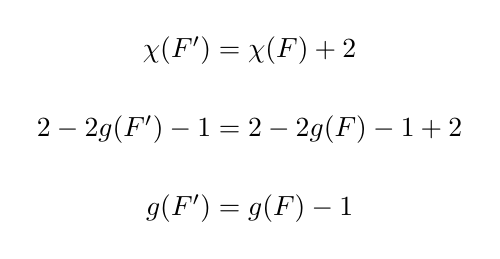
\begin{tikzpicture}
          \node at (0,0) {$\chi(F')=\chi(F)+2$};
          \node at (0, -1) {$2-2g(F')-1=2-2g(F)-1+2$};
          \node at (0, -2) {$g(F')=g(F)-1$};
          \node[rotate=-90] at (0, -0.5) {$\implies$};
          \node[rotate=-90] at (0, -1.5) {$\implies$};
        \end{tikzpicture}
      \end{center}
      co daje sprzeczność z minimalnością $g(F)$.
  \end{itemize}
\end{frame}

\begin{frame}{Genus sumy spójnej}{ciąg dalszy ciągu dalszego dowodu $g(K_1\# K_2)\geq g(K_1)+g(K_2)$}
  \begin{itemize}
    \item Po rozcięciu dostajemy więc dwie rozmaitości: $F'=F''+X$. Wiemy, że 
      $$\chi(F)+2=\chi(F')=\chi(F'')+\chi(X).$$
    \item Rozcinając i wklejając dyszczki nie zmieniliśmy brzegu $F'$, więc $F''$ nadal ma jedną komponentę spójności a $X$ jest zamknięte.
    \item Wiemy więc, że $\chi(X)\leq 2$, a łącząc to z faktem, że $X$ jest zamkniętą powierzchnią wiemy, że $X=S^2$ i $\chi(X)=2$.
  \end{itemize}
\end{frame}

\begin{frame}{Genus sumy spójnej}{koniec ciągu dalszego dowodu $g(K_1\# K_2)\geq g(K_1)+g(K_2)$}
  \begin{itemize}
    \item W takim razie $\chi(F'')=\chi(F)$ i dzielą one również genus.
    \item Powtarzamy historię aż przekrój będzie miał tylko łuczek między dwoma punktami $S\cap K$.
    \item Wtedy umiemy rozciąć nową powierzchnię $F$ rzeczonym łuczkiem, by dostać dwie powierzchnie $F_1$ i $F_2$, których brzegi to odpowiedni $K_1$ i $K_2$.
    \item Po cichu dokleiliśmy kreseczkę, więc
      $$\chi(F)=\chi(F_1)+\chi(F_2)-\chi(\kreska)$$
      $$g(K_1)+g(K_2)\leq g(F_1)+g(F_2)=g(F).$$
  \end{itemize}

  \begin{tikzpicture}[overlay, remember picture]
    \node at (\paperwidth/6 * 5,0) {\includegraphics[width=1cm]{../Donald_Duck.png}};
  \end{tikzpicture}
\end{frame}


\section{Pierwsze zastosowania}

\begin{frame}{Węzły pierwsze}{czyli po co nam te rodzaje, rodziny, rzędy i gromady?}
  \begin{block}{Fakt}
    Jeśli $g(K)=1$, to $K$ jest węzłem pierwszym.
  \end{block}

  \textbf{\color{orange}Dowód}

  Załóżmy, że $K=K_1\# K_2$. Wówczas $g(K_1)+g(K_2)=g(K)=1$. Genus ma to do siebie, że jest $\mathbb{N}$, więc BSO. $g(K_1)=0$ i $K_1$ jest węzłem trywialnym.
\end{frame}

\begin{frame}{Rozkład na węzły pierwsze}
  \begin{theorem}
    Każdy węzeł ma rozkład pierwszy, tzn.
    $$K=K_1\# K_2\# ...\# K_n$$
    gdzie $K_i$, $i=1,..., n$, jest węzłem pierwszym.
  \end{theorem}

  \textbf{\color{orange}Dowód}

  Indukcja po $g(K)$. Jeśli $g(K)=1$ to węzeł jest pierwszy.

  Zakładamy teraz, że umiemy rozłożyć węzły genusu $\leq n$. Niech $g(K)=n+1$, czyli $K$ nie jest węzłem pierwszym. Piszemy $K=K_1\# K_2$, gdzie $g(K_i)\geq 1$ dla obu komponentów. Rozkładamy $K_1$ i $K_2$ i jesteś w domu.
\end{frame}

\begin{frame}{Graf Seiferta}{powtórka}
  \begin{columns}
    \begin{column}{0.5\textwidth}\centering
      \includegraphics[width=\textwidth]{6_1-seifert.png}
    \end{column}
    \begin{column}{0.5\textwidth}\centering
      \begin{tikzpicture}
        \draw[very thick, orange!40!bg-dim] (-1,0) to[out=90, in=180] 
          (2, 2) to[out=0, in=90] 
          (3, 0) to[out=-90, in=0] 
          (2, -2) to[out=180, in=-90]
          (-1, 0);
        \draw[very thick, orange!40!bg-dim] (-1, 0) to[out=45, in=180-45]
          (0.5,0) to[out=180+45, in=-45] (-1, 0);


        \fill[yellow] (0.5,0) circle (6pt);
        \fill[yellow] (-1, 0) circle (6pt);
        \fill[yellow] (3, 0) circle (6pt);

        \fill[blue] (2, 2) circle (6pt);
        \fill[blue] (2, -2) circle (6pt);
      \end{tikzpicture}
    \end{column}
  \end{columns}
  \bigskip 
  \centering
\end{frame}

\begin{frame}{Seifert matrix}{nie-niezmiennik z nieba}
  \begin{columns}
    \begin{column}{0.6\textwidth}
      \begin{tikzpicture}
        \begin{scope}[scale=0.5, shift={(-2, 0)}]
          \draw[very thick, orange!40!bg-dim] (-1,0) to[out=90, in=180] 
            (2, 2) to[out=0, in=90] 
            (3, 0) to[out=-90, in=0] 
            (2, -2) to[out=180, in=-90]
            (-1, 0);
          \draw[very thick, orange!40!bg-dim] (-1, 0) to[out=45, in=180-45]
            (0.5,0) to[out=180+45, in=-45] (-1, 0);


          \fill[yellow] (0.5,0) circle (6pt);
          \fill[yellow] (-1, 0) circle (6pt);
          \fill[yellow] (3, 0) circle (6pt);

          \fill[blue] (2, 2) circle (6pt);
          \fill[blue] (2, -2) circle (6pt);
        \end{scope}

        \node at (2,-2.5) {\includegraphics[width=4cm]{6_1-seifert.png}};
        \draw[very thick] (1.5, -3) to[out=-90, in=180]
          (2, -4) to[out=0, in=-90]
          (3, -3.7) to[out=90, in=180]
          (3.3, -3.2) to[out=0, in=-90]
          (3.7, -2.7) to[out=90, in=0]
          (3.3, -2.2) to[out=180, in=-90]
          (3, -1.7) to[out=90, in=0]
          (2, -1.4) to[out=180, in=90] 
          (1.5, -3);
        \draw[bg-dim, very thick] (1, -2.7) to[out=0, in=-90] 
          (2.2, -2.3) to[out=90, in=0] 
          (1, -1.9) to[out=180, in=90] 
          (0.1, -2.3) to[out=-90, in=180]
          (1, -2.7);

        \node at (1, -3) {$\color{bg-dim}\alpha_1$};
        \node at (3.7, -3) {$\alpha_2$};

      \end{tikzpicture}
    \end{column}
    \begin{column}{0.4\textwidth}
      Cykle w grafie Seiferta powierzchnie Seiferta mają cykle. Przenosimy te cykle, które ograniczają różne obszary grafu na powierzchnię Seiferta.
      \bigskip 

      Spychamy pętelkę $\alpha_i$ do góry pow. S. tak, żeby nie przecinała się z $\alpha_j$ dla wybranego $j$. Po potrząśnięciu nazywamy ją $\alpha_i^{\#}$.
      \bigskip 

      Dostajemy link.
    \end{column}
  \end{columns}
\end{frame}



\begin{frame}{Seifert matrix}{liczymy niebiański nie-niezmiennik}
  Mamy $n$ pętelek. Orientujemy je dowolnie. Możemy stworzyć macierz
  $$\left[ lk(\alpha_i, \alpha_j^{\#} \right]_{i,j=1,...,n},$$
  gdzie $lk(\alpha_i, \alpha_j^{\#})$ oznacza linking number danego linku.
  \medskip 

  Dla węzła $6_1$ z poprzedniego slajdu dostajemy
  $$
  V=\begin{bmatrix}
    -1 & 1\\ 
    0 & 2 
  \end{bmatrix}
  $$
  Macierz ta ma zawsze wymiar $2g(K)\times 2g(K)$.
\end{frame}

\begin{frame}{Sygnatura węzła}{przychodzi z niebiańskiego nie-niezmiennika}
  \begin{definition}
    Jeśli $V$ to macierz Seiferta węzła $K$, to wówczas sygnatura $V+V^T$ (ilość dodatnich wartości własnych - ilość ujemnych) jest niezmiennikiem węzła i nazywa się \textbf{\color{orange}sygnaturą węzła}.
  \end{definition}

  W poprzednim przykładzie sygnatura to $0$, dla lewego trójlistnika to już $-2$, a dla prawego zaś $2$. Zawsze sygnatura odbicia lustrzanego jest przeciwna do oryginalnego węzła.
  \bigskip 

  Możemy pokazać, że sygnatura węzła jest zawsze parzysta.
\end{frame}


\begin{frame}{Ciekawostka}{na dobranoc}
  \begin{definition}
    \textbf{\color{green}Zgodność linków} (ang. \emph{link concordance}) - dwa linki $L_0$ i $L_1$ w $S^n$ są \emph{\color{blue}zgodne}, jeśli istnieje włożenie
    $$f:L_0\times[0, 1]\to S^n$$
    $$f(L_0\times\{0\})=L_0\;i\;f(L_0\times\{1\})=L_1$$
  \end{definition}
  Niezmiennikami tej relacji (która daje grupę abelową) są m.in.
  \begin{itemize}
    \item linking number
    \item sygnatura węzła (wrócimy, obiecuję)
    \item niezmienniki Milnora $\heartsuit$.
  \end{itemize}
\end{frame}

\end{document}


  % \begin{center}
  %   \begin{tikzpicture}
  %     %\node[rotate=-90, opacity=0.3] at (0,0) {\includegraphics[width=4cm]{6_1.png}};
  %
  %     \begin{scope}
  %       \coordinate (a1) at (2, 0);
  %       \coordinate (a2) at (1.2, 0);
  %       \coordinate (a3) at (1.4, 1.5);
  %       \coordinate (a4) at (1.4, -1.5);
  %       \coordinate (a5) at (-1,0.5);
  %       \coordinate (a6) at (-1,-0.5);
  %       \coordinate (a7) at (-1, -1.5);
  %       \coordinate (a8) at (-1, 1.5);
  %       \coordinate (a9) at (0.7, -.7);
  %       \coordinate (a10) at (0.7, .7);
  %
  %
  %       \begin{knot}[
  %         background color=bg0,
  %         clip width=5pt,
  %         ignore endpoint intersections=false,
  %         %draft mode=crossings,
  %         flip crossing=4,
  %         flip crossing=2,
  %         flip crossing=6
  %         ]
  %         \strand[->] (a1) to[out=-90, in=30] (a9);
  %         \strand[->] (a9) to[out=210, in=0, looseness=1.3] (a7);
  %         \strand[->] (a7) to[out=180, in=210] (a5);
  %         \strand[->] (a5) to[out=30, in=180] (a4);
  %         \strand[->] (a4) to[out=0, in=-90] (a2);
  %         \strand[->] (a2) to[out=90, in=0] (a3);
  %         \strand[->] (a3) to[out=180, in=-30] (a6);
  %         \strand[->] (a6) to[out=150, in=180, looseness=1.3] (a8);
  %         \strand[->] (a8) to[out=0, in=150] (a10);
  %         \strand[->] (a10) to[out=-30, in=90] (a1);
  %       \end{knot}
  %     \end{scope}
  %
  %     \begin{scope}[shift={(5, 0)}]
  %       \coordinate (a1) at (2, 0);
  %       \coordinate (a2) at (1.2, 0);
  %       \coordinate (a3) at (1.4, 1.5);
  %       \coordinate (a4) at (1.4, -1.5);
  %       \coordinate (a5) at (-1,0.5);
  %       \coordinate (a6) at (-1,-0.5);
  %       \coordinate (a7) at (-1, -1.5);
  %       \coordinate (a8) at (-1, 1.5);
  %       \coordinate (a9) at (0.7, -.7);
  %       \coordinate (a10) at (0.7, .7);
  %
  %       %\foreach \i in {1,..., 10} \fill (a\i) circle (2pt) node[above] {\i};
  %       \draw[name path=l1, ->] (a1) to[out=-90, in=30] (a9);
  %       \draw[name path=l2, ->] (a9) to[out=210, in=0, looseness=1.3] (a7);
  %       \draw[name path=l3, ->] (a7) to[out=180, in=210] (a5);
  %       \draw[name path=l4, ->] (a5) to[out=30, in=180] (a4);
  %       \draw[name path=l5, ->] (a4) to[out=0, in=-90] (a2);
  %       \draw[name path=l1, ->] (a1) to[out=-90, in=30] (a9);
  %       \draw[name path=l6, ->] (a2) to[out=90, in=0] (a3);
  %       \draw[name path=l7, ->] (a3) to[out=180, in=-30] (a6);
  %       \draw[name path=l8, ->] (a6) to[out=150, in=180, looseness=1.3] (a8);
  %       \draw[name path=l9, ->] (a8) to[out=0, in=150] (a10);
  %       \draw[name path=l10, ->] (a10) to[out=-30, in=90] (a1);
  %     \end{scope}
  %   \end{tikzpicture}
  % \end{center}
